Énoncer puis démontrer les formules d'addition en trigonométrie

\section{Cours}
Les formules d'addition en trigonométrie sont :
$$\cos(a + b) = \cos(a)\cos(b) - \sin(a)\sin(b)$$
$$\sin(a + b) = \sin(a)\cos(b) + \sin(b)\cos(a)$$

\section{Démonstration}
Soit un cercle trigonométrique dans le repère $(O, \vec{i}, \vec{j})$.\\
Soient trois points $M$, $M'$ et $N$ du cercle tels que :
\begin{itemize}
    \item $M$ tel que $(\vec{OI}, \vec{OM}) = a\,(2\pi)$
    \item $M'$ tel que $(\vec{OI}, \vec{OM'}) = a + b\,(2\pi)$
    \item $N$ tel que $(\vec{OM}, \vec{ON}) = \frac{\pi}{2}\,(2\pi)$
\end{itemize}
    
    \begin{center}
        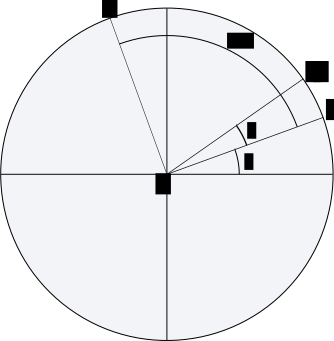
\includegraphics[scale=.75]{cercle.pdf}
    \end{center}
Le point $M'$ dans le repère orthonormal $(O, \vec{OM}, \vec{ON})$ est tel que $(\vec{OM}, \vec{OM'}) = b\,(2\pi)$.\\
Donc :
\begin{equation}
    \label{vec-OM}
    \vec{OM'} = \cos(b)\vec{OM} + \sin(b)\vec{ON}
\end{equation}

Or dans le repère $(O, \vec{i}, \vec{j})$ on a :
\begin{itemize}
    \item $\vec{OM} = \cos(a)\vec{i} + \sin(a)\vec{j}$
    \item $\vec{ON} = \cos(a + \frac{\pi}{2})\vec{i} + \sin(a + \frac{\pi}{2})\vec{j} = -\sin(a)\vec{i} + \cos(a)\vec{j}$ car $\cos(a + \frac{\pi}{2}) = -\sin(a)$ et $\sin(a + \frac{\pi}{2}) = \cos(a)$.
\end{itemize}

\begin{eqnarray}
   (1) & \Leftrightarrow & \vec{OM} = \cos(b) \times (\cos(a)\vec{i} + \sin(a)\vec{j}) + \sin(b)(-\sin(a)\vec{i} + \cos(a))\vec{j} \\
    & \Leftrightarrow & \color{green}{(\cos(a)\cos(b) - \sin(a)\sin(b))}\vec{i} + \color{blue}{(\sin(a)\cos(b) + \sin(b)\cos(a))}\vec{j}
\end{eqnarray}

Or dans le repère orthonormal $(O, \vec{i}, \vec{j})$,\\
$\vec{OM'}$ a pour coordonnées $\color{green}{\cos(a + b)}\vec{i} + \color{blue}{\sin(a+b)}\vec{j}$.
Par identification, on en déduit donc les relations cherchées :
$$\cos(a + b) = \cos(a)\cos(b) - \sin(a)\sin(b)$$
$$\sin(a + b) = \sin(a)\cos(b) + \sin(b)\cos(a)$$
    
CQFD.
